%%% -*- coding: utf-8 -*-
\newpage

\chapter{Background}
\label{chap:background}

\section{Poker Foundations}
\label{sec:foundations}

Texas Hold'em poker variant starts with every player receiving 2 private cards. Then, there is a betting round: every player bets some amount that they have the best hand. This first round is called \textbf{pre-flop}.

Next, 3 public cards are dealt to the table. This is called \textbf{flop}. The flop is public, and those 3 cards are shared among all players. A betting round happens again, but now the players bet who has the best combination of private hand and shared table, a total of 5 cards. Every bet goes to the table pot.

Afterward, there is the \textbf{turn} round. A card is dealt to the table, followed by a betting round. Finally, another card is dealt to the table - the \textbf{river} round - and the last betting round finishes the game.

A player with the best combination of private and public cards wins the pot. Also, a player wins if all other players have given up. In case of tie, winners share the table pot.
 
The bet can be a fold, a call of the previous bet or a raise. When a player folds, he is out of this game and loses the amount he has previously given to the table pot. Each player announces it's bet starting from the first player after the dealer until every player but one fold or every active player bet the same amount (call). 

\vspace{2cm}
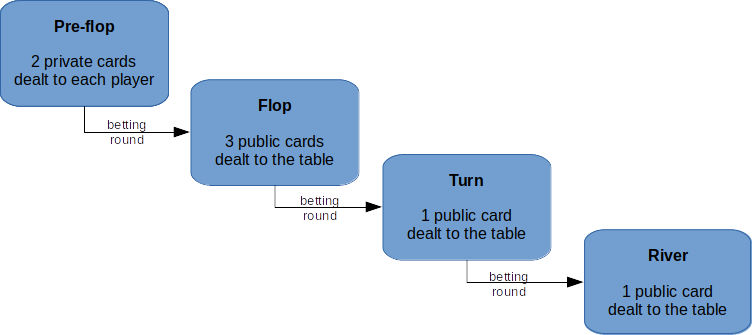
\includegraphics[scale=2]{poker-foundations}
\vspace{0.5cm}

\subsection{Hand Ranking}

The hands are listed bellow in ranking order:

High card: all five cards of different rank and a variety of suits;

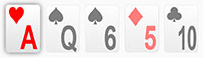
\includegraphics[scale=2]{high-card}

One pair: two cards of the same rank and three different cards;
  
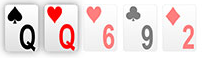
\includegraphics[scale=2]{pair}

Two pairs: two pairs and one different card;

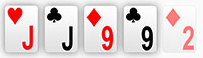
\includegraphics[scale=2]{two-pairs}
  
Three of a kind: three cards of the same rank and two different cards;
  
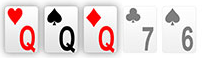
\includegraphics[scale=2]{three-of-a-kind}

Straight: five cards in sequence of rank with different suits;
  
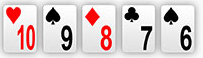
\includegraphics[scale=2]{straight}
  
Flush: five cards of the same suit;
  
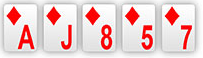
\includegraphics[scale=2]{flush}
  
Full House: three cards of the same rank and two cards of the same rank;
  
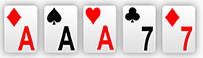
\includegraphics[scale=2]{full-house}
  
Four of a kind: four cards of the same rank;
  
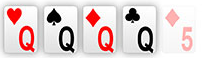
\includegraphics[scale=2]{four-of-a-kind}
  
Straight flush: a straight of the same rank;
  
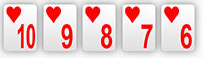
\includegraphics[scale=2]{straight-flush}
 
If two players have the same type of hand, the hand with higher card wins. A player can use a combination of its private cards and the public cards in the table. In the end, a player has 7 cards available but can combine only 5 in a poker hand.

\subsection{Positions}
\label{sec:positions}

It is trivial to understand that player's position matters. The last player to bet have more information about other players' bets and can take a better decision in order to maximize its rewards.

In each round, each player is the \textbf{dealer} of the deck, in sequence. The player next to the dealer is the \textbf{small-blind} and the next player is the \textbf{big-blind}. In pre-flop, the small-blind have to place a minimum bet and the big-blind has to place twice the small-blind. To participate, every player has to bet as least the big-blind amount. In the next round, the flop, bets start from zero.

In this work, we will consider a game of 5 players, therefore, there will be 5 positions, and each player will be dealer, small-blind, and big-blind, once every 5 games.

\subsection{Actions}

Given a state of the game, a player can

\begin{itemize}
  \item \textbf{Bet}: to place an amount to the pot when no one has done it before
  \item \textbf{Raise}: to raise a previous bet
  \item \textbf{Call}: to bet the same amount of a previous bet
  \item \textbf{Fold}: to give up, and lose the money placed in the pot
  \item \textbf{Check}: when no bet has been made, a player can pass (it's the same as betting an amount of 0)
\end{itemize}

Also, in no-limit poker a player can bet all of its money. This is called \textbf{all-in}

\subsection{Variants}
Poker variants usually differ in orthogonal dimensions. The two most common are number of players and betting structure.

A \textbf{heads-up} variant includes two players. The \textbf{ring} variant includes more than two players and we will refer to it as multiplayer variant. This work concerns about multiplayer poker but can be extended to the heads-up variant.

In the \textbf{limit} variant, also called \textit{fixed limit}, the players can only raise to a fixed amount, usually the big-blind amount or twice the big-blind. In \textbf{no-limit} poker, a raise can be anything from the last bet to the players total stack.

\section{Related Work}
\label{chap:related-work}

The first computer program to play poker was called Orac, and was created by Mike Caro to compete in World Series of Poker in 1984.

Afterward, University of Alberta, Carnegie Mellon and University of Auckland led the development of poker bots.

In 1998, the Computer Poker Research Group at University of Alberta, led by Michael Bowling, released Loki, an artificial intelligence capable of playing Limit Heads-Up Texas Hold’em ~\cite{Billings2016}. Next, they improved their work and created Poki, in 2000 ~\cite{Davidson2000}. Both of them focused in modeling the opponent’s strategy, but still relied in “search” by simulation to find the best decision.

In 2003, scientists began to shift from the chess methodology model, and in 2008 a poker bot developed in University of Alberta, called Polaris, played 6 heads up No Limit Hold’em matches against humans, with 3 wins, 2 losses and 1 tie.

Next, in 2009, University of Auckland introduced Sartres, its first poker AI. It was designed to play specifically heads up Limit Texas Hold’em, and was the first one to use a case-based reasoning methodology ~\cite{Rubin2009}.

Counterfactual Regret Minimization started to play a big whole in this field ~\cite{Zikenvich2008}, and Limit Texas Hold’em was essentially solved in 2015, by Cepheus, another AI developed at the Computer Poker Research Group at University of Alberta ~\cite{Bowling2008}.

Also in 2015, a professor at Carnegie Mellon University developed Claudico ~\cite{Brown2015}, a No Limit Texas Hold’em bot, but it lost heads up matches against pro players. It required  a Pittsburgh supercomputer with 16 terabytes of RAM to learn the its strategy.

Libratus succeeded Claudico, but was rewritten from scratch. It was build with more than 15 million core hours of computation, compared to 3 million performed for Claudico. It applied a new variant of Counterfactual Regret Minimization, namely CFR+, developed by Oskari Tammelin, a scientist involved in the Cepheus project ~\cite{Brown2017}.

In 2016 David Silver introduced Neural Fictitious Self Play, a deep reinforcement learning method composed of two neural networks that learn approximate Nash equilibria of imperfect-information games. Silver's goal was to not rely on engineering abstractions or any domain knowledge, and still be capable of learning in a complex environment. It was applied to Limit Texas Hold'em and approached the performance of state-of-the-art~\cite{Silver2016}.

Finally, in 2017 the Computer Research Group (UoA) together with several scientists from the Czech Republic, introduced DeepStack, an algorithm for imperfect information scenarios. This work combined many different deep learning strategies, like recursive reasoning, to handle information asymmetry, decomposition to focus computation on the relevant decision, and a form of intuition algorithm to automatically learn from self-play ~\cite{Moravcik2017}. For the first time, a computer program defeated with statistical significance professional poker players in heads-up no-limit Texas Hold’em.

%%% Local Variables:
%%% mode: latex
%%% TeX-master: thesis.tex
%%% End:
